\subsubsection*{1.a}
Insertion dans la table users 

\lstinputlisting[style=sqlstyle]{SQL/Partie3/users.sql}

\begin{center}
    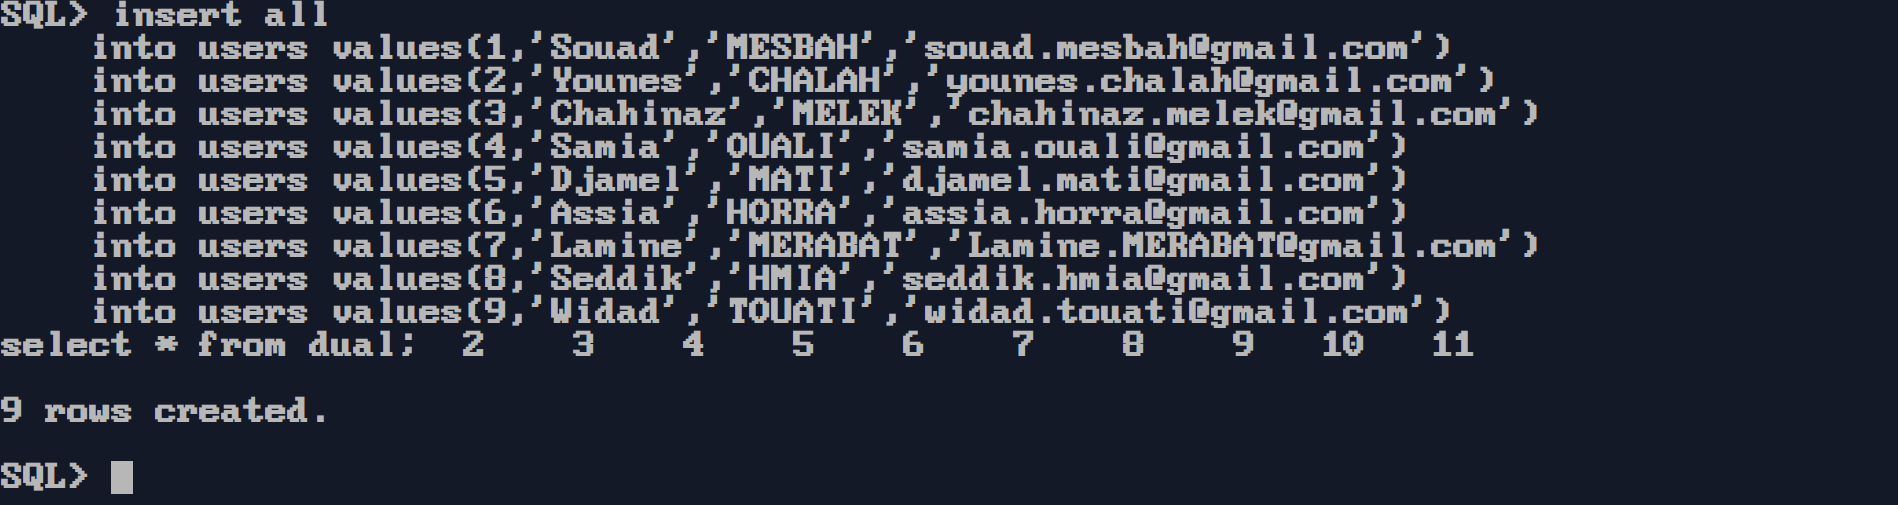
\includegraphics[width=\textwidth]{ScreenShot/Partie3/users.png}
\end{center}

\vspace{0.25cm}
\subsubsection*{1.b}
Insertion dans la table service

\lstinputlisting[style=sqlstyle]{SQL/Partie3/service.sql}

\begin{center}
    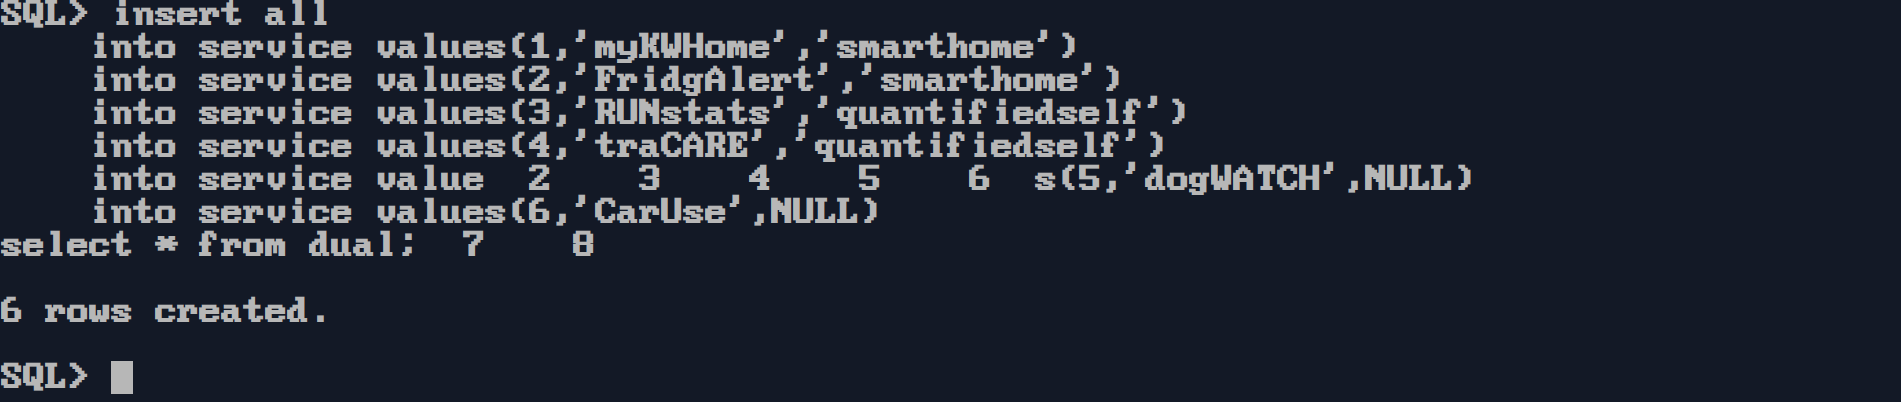
\includegraphics[width=\textwidth]{ScreenShot/Partie3/service.png}
\end{center}

\vspace{0.25cm}
\subsubsection*{1.c}
Insertion dans la table thing 

\lstinputlisting[style=sqlstyle]{SQL/Partie3/thing.sql}

\begin{center}
    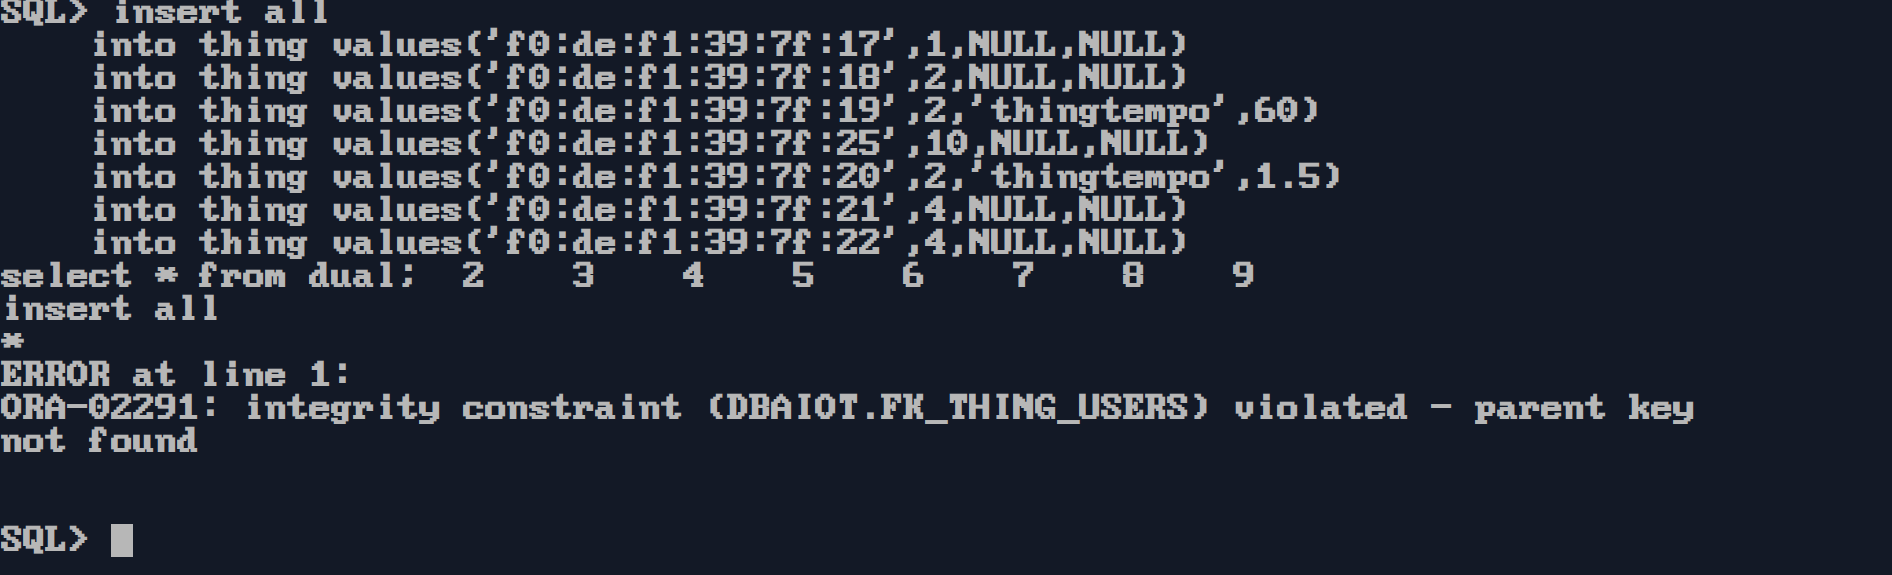
\includegraphics[width=\textwidth]{ScreenShot/Partie3/thing.png}
\end{center}

\begin{prettyBox}{}{myblue}
Le problème rencontré est qu'on a enfreint la contrainte FK\_THING\_USERS, car iduser = 10 n'existe pas dans la table users.
\end{prettyBox}

\vspace{0.25cm}
\subsubsection*{1.d}
Insertion dans la table subscribe

\lstinputlisting[style=sqlstyle]{SQL/Partie3/sub.sql}

\begin{center}
    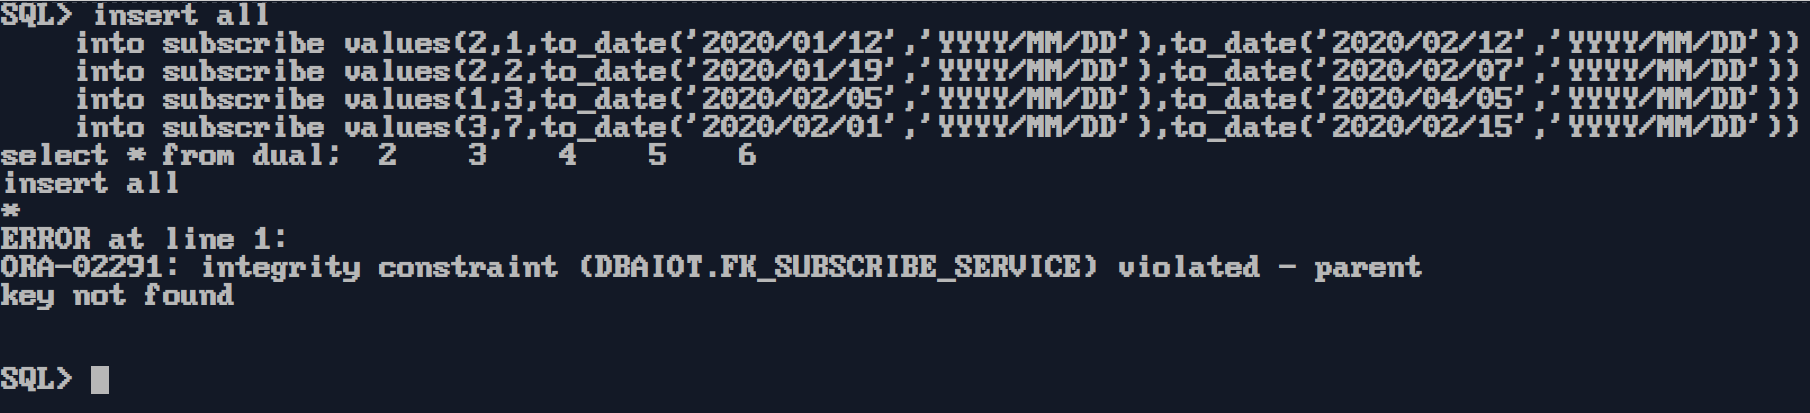
\includegraphics[width=\textwidth]{ScreenShot/Partie3/sub.png}
\end{center}

\begin{prettyBox}{}{myblue}
Le problème rencontré est qu'on a enfreint la contrainte FK\_SUBSCRIBE\_SERVICE, car idservice = 7 n'existe pas dans la table service.
\end{prettyBox}



